\chapter{Teszteredmények}
Ebben a fejezetben a tesztelése menete, a tesztelés által elért eredmények kerülnek bemutatásra.
Mivel esetemben egy meglévő szoftver rendszer továbbfejlesztéséről beszélhetünk, ezért az új funkciók letesztelésén kívül fontos az eddigi funkcionalitás újratesztelése is.
Éppen ezért a tesztesetek alapvetően három részre bonthatóak:
\begin{itemize}
\item A determinisztikus throughput maximalizáló tesztelése
\item A sztochasztikus alapesetek (1-1) tesztelése
\item A sztochasztikus multiproduct esetek tesztelése
\end{itemize}
A teszteléshez használt input fájlok megtalálhatóak a CD melléklet \fileName{Tesztelés/Tesztfájlok} mappájában.
Ezen inputfájlok tartalma, nevezetesen a termékekre, illetve a forgatókönyvekre vonatkozó paraméterek random szám generátorral készültek adott tartományokon belül.
A tesztkonfigurácó leírása:
\begin{itemize}
\item Windows 7 operációs rendszer 
\item Qt 5.11.2, Microsoft Visual C++ Compiler 15.0, Boost Libraries 1.68.0
\item Intel i5 3570K 3,8 Ghz processzor
\item 8 GB RAM
\end{itemize}
\section{A determinisztikus throughput maximalizáló tesztelése}
A determinisztikus throughput maximalizáló teszteléséhez használt teszt fájlok a CD melléklet  \fileName{Tesztelés/Tesztfájlok/Determinisztikus} mappájában találhatóak, míg a teszteredményeket rögzítő \fileName{DeterministicTestResults.ods} fájl a CD melléklet \fileName{Tesztelés/Teszteredmények} mappájában található.
A determinisztikus teszt fájlokban található termékek profit értékei véletlenszerűen választott számok, a többi adat pedig a \fileName{multipurpose.ods} fájlból került átmásolásra.
A \ref{deterministic_test} ábrán látható egy példa egy determinisztikus teszt fájlra.
\begin{figure}[H]
\begin{center}
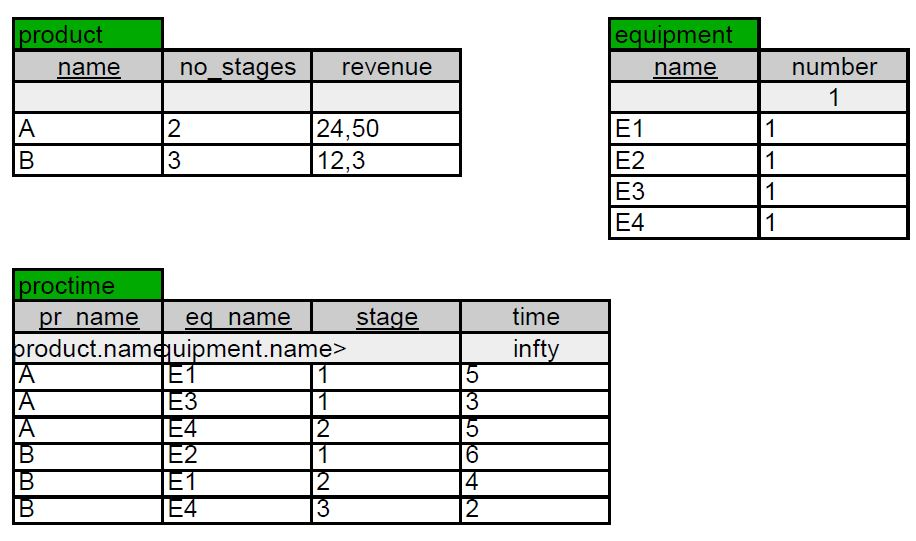
\includegraphics[scale=0.5]{deterministicTest}
\caption{Példa egy determinisztikus teszt fájlra}
\label{deterministic_test}
\end{center}
\end{figure}
Ezen fájlt felhasználva a determinisztikus throughput maximalizáló 15 óra időhorizont érték mellett 61.3 profit egységet adott eredményül a következő gyártott mennyiségek mellett: $2A+1B$.
Jól látható, hogy az eredmény helyes, hiszen $2 \cdot 24.5 +12,3=61.3$.
Ezenfelül a solver master git branchén található verziót futtatva (melyhez a dolgozat írásakor még nem került hozzáadásra a munkám) szintén megegyező eredményt kapunk, mind a profit értékeket, mind a kimeneti ütemterveket figyelembe véve, valamint a futási időkben sem figyelhető meg számottevő változás.
Ezen adatokat figyelembe véve kijelenthető tehát, hogy a determinisztikus throughput maximalizáló továbbra is hibátlanul működik.     
\section{A sztochasztikus alapesetek tesztelése (1-1)}
\section{A sztochasztikus multiproduct receptek tesztelése}